\capitulo{3}{Conceptos teóricos}
\setcounter{secnumdepth}{3}

\section{Epidemia, pandemia y epidemiología}
En este trabajo, aunque el enfoque principal es el modelado de epidemias, se utilizarán los términos \textit{epidemia} y \textit{pandemia} de manera indistinta, dado que los modelos deterministas que se aplican no distinguen explícitamente entre ambos conceptos. Estos modelos se limitan a simular la dinámica de transmisión de una enfermedad en una población, sin considerar directamente la escala geográfica o el alcance global del brote.
No obstante, es importante señalar que, aunque estos modelos  pueden aplicarse tanto a epidemias como a pandemias, los términos no deben considerarse sinónimos, ya que su diferenciación radica en el contexto y la magnitud del fenómeno. Además, se analizarán situaciones reales que incluyen casos de ambos tipos, aprovechando la versatilidad de los modelos utilizados.

A continuación se definen ambos términos.

\subsection{Epidemia}
Una epidemia es la aparición de una enfermedad en una comunidad, zona o país durante un periodo de tiempo determinado, que afecta de forma simultánea y constante, a un número elevado de personas. En la figura se ve como afecta solo a un país  \ref{fig:epidemia}\footnote{Obtenido de \cite{bbc_ebola_2014}}. Las causas pueden ser diversas e incluyen agentes infecciosos como virus, bacterias, parásitos u hongos, así como factores ambientales y sociales que favorecen la transmisión de la enfermedad. Se considera epidemia cuando cualquier enfermedad infecciosa se descontrola temporalmente y afecta a una proporción significativa de la población.

\begin{figure}[H]
    \centering
    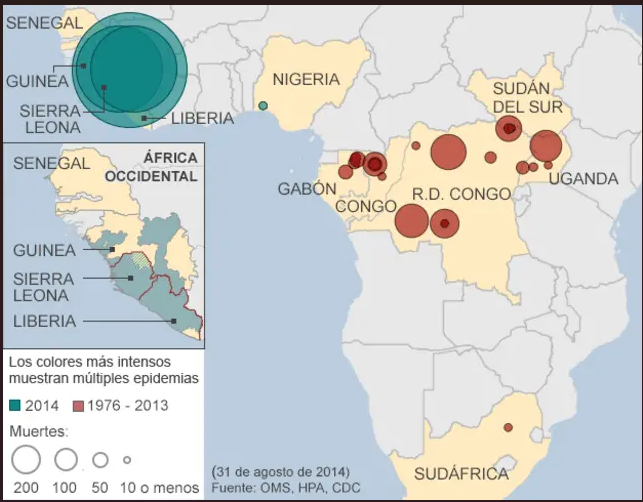
\includegraphics[width=0.7\textwidth]{img/epidemia.png}
    \caption{Ejemplo de epidemia, Ébola.}
    \label{fig:epidemia}
\end{figure}


Cabe destacar que no todas las epidemias son provocadas por enfermedades contagiosas. Aunque muchas se deben a infecciones que se transmiten entre personas, también pueden originarse por factores como el comportamiento humano, el entorno, vectores (como mosquitos) o enfermedades zoonóticas transmitidas por animales. Incluso enfermedades no transmisibles, como la obesidad o la diabetes, pueden alcanzar niveles epidémicos debido a cambios en los estilos de vida.


\subsection{Pandemia}
Una pandemia es una epidemia que se ha propagado a nivel mundial, afectando a un gran número de personas en varios países y continentes. Se caracteriza por la transmisión sostenida de persona a persona y genera un impacto significativo en la salud pública global, en la economía y la estructura social \cite{dias2024towards}. En la figura \ref{fig:pandemia}\footnote{Obtenido de \cite{isglobal_coronavirus_orden}} se puede observar como una pandemia afecta a novel global

\begin{figure}[H]
    \centering
    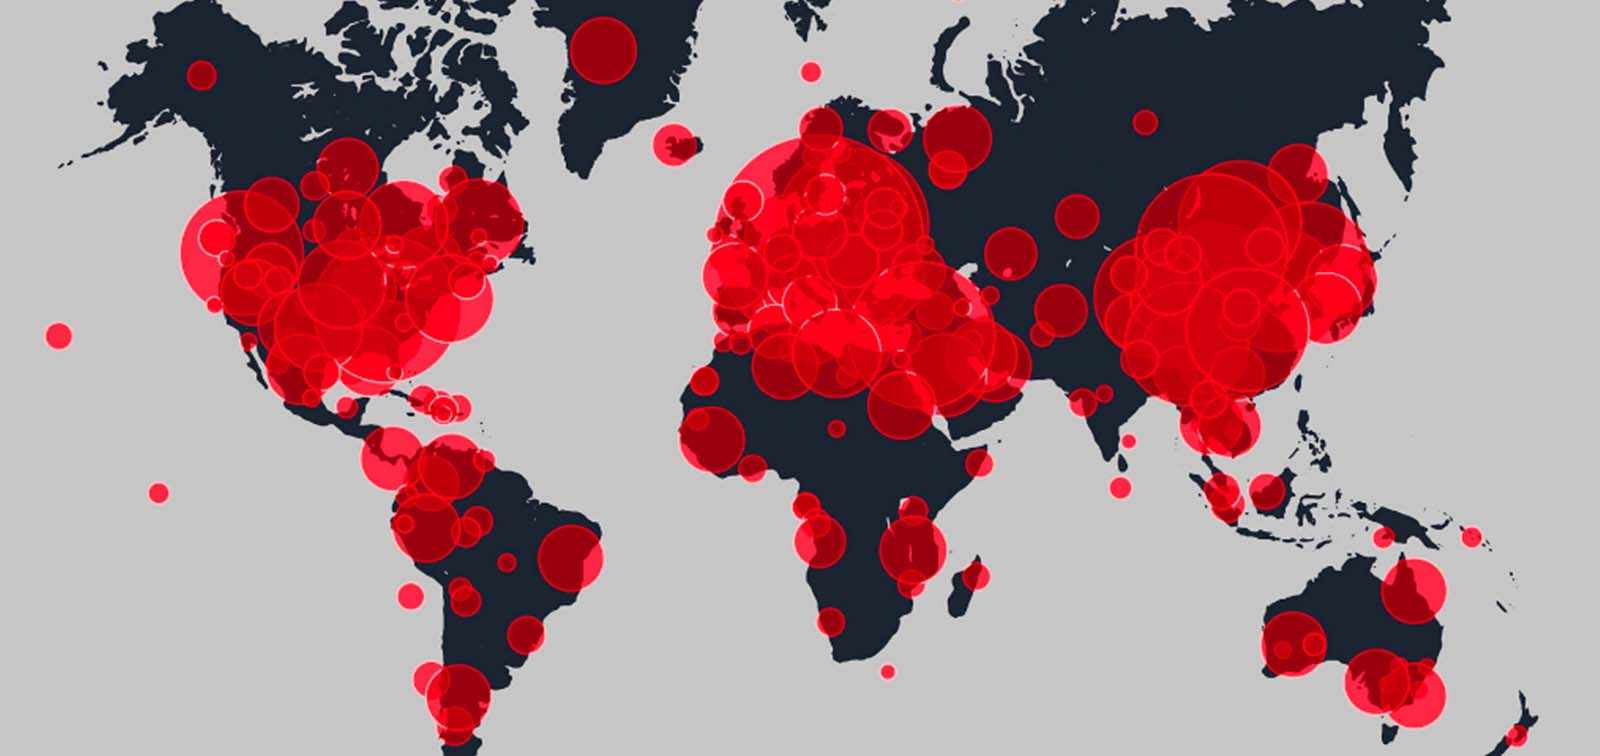
\includegraphics[width=0.7\textwidth]{img/pandemia.jpg}
    \caption{Ejemplo de pandemia, COVID-19.}
    \label{fig:pandemia}
    \vspace{0.5cm} % Ajusta el espacio vertical entre la imagen y el texto
\end{figure}

\subsection{Grupos vulnerables ante las epidemias}
Las epidemias afectan de manera desigual factores sociales, económicos y biológicos. Según \cite{nasution2021poblaciones} entre los más vulnerables se encuentran :
\begin{itemize}
  \item Personas mayores de 60 años, debido al mayor riesgo de complicaciones.
  \item Personas con inmunodeficiencia, ya sea adquirida o congénita.
  \item Mujeres embarazadas, por los cambios fisiológicos que afectan al sistema inmunológico.
   \item Personas con obesidad.
   \item Personas con enfermedades crónicas, como diabetes, enfermedades cardiovasculares, renales, hepáticas o pulmonares.
   \item Grupos socioeconómicos desfavorecidos, que presentan limitaciones en el acceso a servicios de salud y viven en condiciones precarias. 
\end{itemize}

\subsection{Gestión, control y prevención de epidemias}
La gestión de una epidemia requiere de diversas etapas y estrategias. La detección temprana y la vigilancia epidemiológica son fundamentales para identificar brotes y evitar su propagación. Las evaluaciones de riesgo y vulnerabilidad permiten determinar las áreas y poblaciones más afectadas. La preparación incluye la planificación de recursos, la formación del personal y la implementación de sistemas de alerta temprana.

Entre las estrategias preventivas y de control se encuentran la vacunación, el tratamiento y la mejora de las condiciones de saneamiento e higiene. La respuesta eficaz a una epidemia exige la coordinación entre distintos gobiernos, organizaciones internacionales y comunidades locales. Para erradicar la enfermedad, pueden llevarse a cabo campañas masivas de vacunación y otras intervenciones a largo plazo. Un enfoque holístico \cite{tsagkarliotis2023holistic}, que integre factores médicos, sociales, económicos, psicológicos y ambientales, resulta clave para mejorar la prevención y respuesta ante epidemias mediante la aplicación de prácticas innovadoras y enfoques interdisciplinarios. 

Los tratamientos varían según el patógeno. Entre las principales medidas de prevención y control que propone \cite{ministeriosanidad2021} se incluyen:
\begin{itemize}
  \item \textbf{Vacunación}, como herramienta fundamental en la prevención de enfermedades transmisibles.
  \item \textbf{Distanciamiento social y cuarentena}, para limitar el contacto entre personas y reducir la transmisión.
  \item \textbf{Higiene y saneamiento}, mediante el uso de mascarillas, el lavado de manos y la mejora del entorno sanitario.
  \item \textbf{Educación y comunicación}, para informar a la población sobre síntomas, prevención y medidas de respuesta.
  \item \textbf{Refuerzo del sistema de salud}, con inversión en recursos humanos, equipamiento e infraestructuras.
\end{itemize}

\subsection{Ejemplos de epidemias y pandemias a lo largo de la historia}
A lo largo de la historia, distintas epidemias han dejado una huella significativa en la sociedad y la salud pública. Algunos ejemplos relevantes son:
\begin{enumerate}
    \item \textbf{La Peste Negra (1347-1351)}: pandemia de peste bubónica causada por la bacteria \textit{Yersinia pestis}, que provocó la muerte de entre 25 y 30 millones de personas en Europa, aproximadamente un tercio de la población, según \cite{patterson2021societal}. Sus consecuencias económicas y sociales fueron profundas, incluyendo transformaciones en la estructura feudal y escasez de mano de obra. 
    
    \item \textbf{La gripe española (1918-1919)}: provocada por el virus de la influenza A H1N1, infectó a un tercio de la población mundial y causó la muerte de aproximadamente 50 millones de personas. La alta mortalidad se debió a la falta de tratamientos efectivos y a la sobrecarga de los sistemas de salud. Impulsó el desarrollo de los primeros sistemas de vigilancia epidemiológica \cite{kilbourne2006influenza}.
    
  
    \item \textbf{VIH/SIDA (desde 1981)}: el virus de la inmunodeficiencia humana ha causado una pandemia global que ha provocado más de 26 millones de muertes. Ha tenido un impacto desproporcionado en regiones como África subsahariana, aunque se han logrado importantes avances en investigación, prevención y tratamiento \cite{miranda2022tale}.
    \item \textbf{Ébola (2013-2016)}: el brote en África Occidental causó alrededor de 11000 muertes y colapsó los sistemas de salud locales. La respuesta internacional incluyó el desarrollo de tratamientos y vacunas, así como mejoras en infraestructuras sanitarias \cite{who2014ebola}.
    \item \textbf{COVID-19 (desde 2019)}: causada por el virus SARS-CoV-2, ha provocado millones de muertes y ha tenido un impacto sin precedentes en la salud pública, la economía y la vida cotidiana. Ha subrayado la importancia de la preparación ante emergencias, la cooperación internacional y la rápida implementación de medidas de salud pública. Se ve en la figura \ref{fig:covid} obtenida de \cite{bbc2020corea} como se vestían los especialistas para realizar prubas y no contagiarse
    
    \begin{figure}[H]
        \centering
        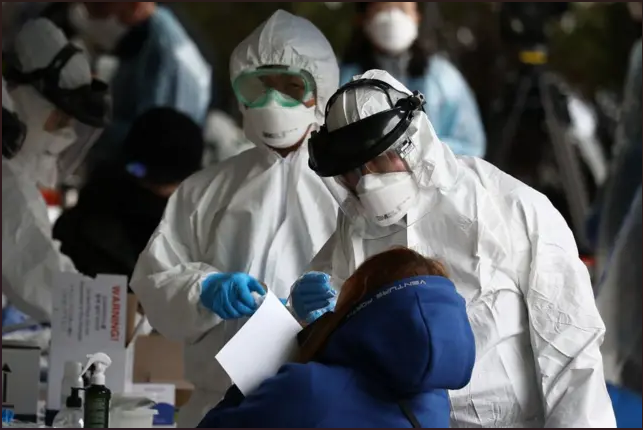
\includegraphics[width=0.7\textwidth]{img/covid.png}
        \caption{Realización de pruebas y vestimenta durante la pandemia}
        \label{fig:covid}
        \vspace{0.5cm} % Ajusta el espacio vertical entre la imagen y el texto
    \end{figure}
\end{enumerate}

\subsection{Epidemiología}
La epidemiología es la ciencia que estudia la distribución y los determinantes de los eventos relacionados con la salud en poblaciones específicas, así como la aplicación de ese conocimiento para la prevención y control de problemas de salud. Se enfoca en identificar factores de riesgo, causas de enfermedades y en desarrollar e implementar intervenciones para su control \cite{hajat2010introduction}.

En el contexto de las epidemias, la epidemiología permite investigar brotes infecciosos localizados en tiempo y espacio, facilitando la identificación de la fuente, el riesgo y los mecanismos de transmisión, como se describe \cite{riley2019differentiating}. En el caso de las pandemias, la epidemiología adquiere una dimensión global, evaluando la propagación de enfermedades en múltiples países, según \cite{piret2021pandemics}. 

Resulta crucial para la identificación, prevención y control de epidemias y pandemias. A través de sus métodos de investigación, permite comprender la distribución de las enfermedades, identificar sus causas y diseñar intervenciones eficaces para proteger la salud pública.

\subsection{Endemia}
Una endemia según \cite{ranm_endemia} es una enfermedad que se mantiene presente de forma constante en una población o región geográfica específica. A diferencia de una epidemia o pandemia, no hay un aumento de casos, sino que los niveles de contagio son relativamente estables y previsibles con el tiempo.

En la figura \ref{fig:difernecias}\footnote{Obtenida de \cite{rie2020covid}}, se muestra de forma visual las diferencias entre los conceptos de endemia, epidemia y pandemia.


\begin{figure}[H]
        \centering
        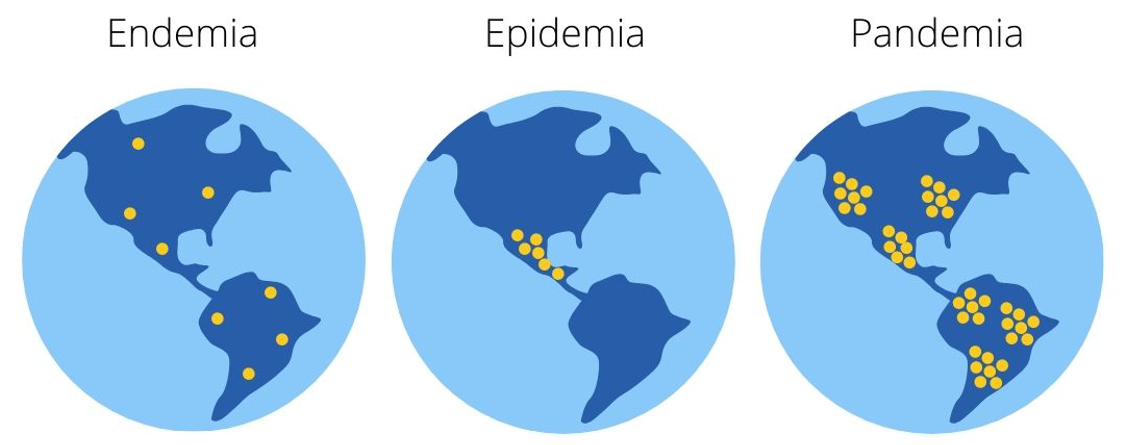
\includegraphics[width=0.7\textwidth]{img/endemia.png}
        \caption{Diferencias entre epidemia, endemia y pandemia.}
        \label{fig:difernecias}
        \vspace{0.5cm} % Ajusta el espacio vertical entre la imagen y el texto
    \end{figure}


\section{Modelos epidemiológicos  deterministas}
\subsection{Modelos epidemiologícos}
Los modelos epidemiológicos son herramientas matemáticas y computacionales que permiten representar de manera simplificada los procesos biológicos, sociales y ambientales que influyen en la propagación de enfermedades dentro de una población. Estos modelos describen cómo las enfermedades infecciosas (y, en algunos casos, no infecciosas) se transmiten entre individuos y cómo varía el estado de salud de la población a lo largo del tiempo.

En términos generales, un modelo epidemiológico intenta captar las dinámicas clave del contagio, recuperación, inmunidad, nacimiento y muerte, mediante el uso de ecuaciones diferenciales, teoría de probabilidades o simulaciones computacionales. Dependiendo de su complejidad, pueden incorporar factores como heterogeneidad en la población, movilidad, redes de contacto, y respuesta a intervenciones sanitarias.

Entre los objetivos principales de los modelos epidemiológicos se encuentran:
\begin{itemize}
    \item Describir la dinámica de transmisión de enfermedades en poblaciones susceptibles, entender cómo y por qué una enfermedad se propaga o desaparece.
    \item Estimar parámetros clave como la duración de la infección, la tasa de transmisión, número básico de reproducción R0 y la proporción de población que debe ser vacunada para llegar a alcanzar la inmunidad colectiva.
    \item Explorar escenarios hipotéticos, permitiendo simular diversas condiciones y prever la evolución en el tiempo de una epidemia bajo diferentes supuestos.
    \item Evaluar estrategias de intervención y control como vacunación, cuarentena, aislamiento de casos, uso de mascarillas, cierre de escuelas. permiten calcular el impacto potencial de estas medidas antes de aplicarlas.
    \item Guiar decisiones en salud pública, ofreciendo soporte cuantitativo para la toma de decisiones en contextos de brotes, pandemias o planificación preventiva.
    \item Comprender el impacto de factores sociales y demográficos, como la densidad poblacional, la movilidad geográfica, la estructura etaria o el comportamiento humano, sobre la propagación de enfermedades.
    \item Contribuir al diseño de políticas sanitarias efectivas, mediante la identificación de puntos críticos donde las intervenciones pueden ser más eficaces o eficientes.
\end{itemize}

Los modelos epidemiológicos pueden clasificarse, entre otros criterios, según la ausencia o presencia de aleatoriedad:
\begin{itemize}
    \item \textbf{Deterministas}, aquellos en los que la evolución del fenómeno depende de manera unívoca del conjunto de condiciones iniciales y de los parámetros establecidos. Es decir, no existe aleatoriedad en el proceso, si se repite el modelo con los mismos valores, el resultado será siempre el mismo. Este tipo de modelos se basa habitualmente en ecuaciones diferenciales y resulta útil para analizar el comportamiento general de una enfermedad en poblaciones grandes, donde se busca una aproximación global y reproducible de un fenómeno.
    \item \textbf{Estocásticos}, incorporan procesos aleatorios, lo que implica que, aun con el mismo conjunto de variables y parámetros, la solución del modelo puede variar en cada ejecución. Esto permite captar mejor la variabilidad inherente a fenómenos reales, especialmente en contextos donde las poblaciones son pequeñas o existe un alto grado de incertidumbre.
\end{itemize}
	
Para el desarrollo del este trabajo se ha elegido el uso de modelos deterministas, dado que permiten describir de manera clara y estructurada la evolución de una enfermedad en función de condiciones iniciales y parámetros conocidos. Este enfoque facilita el análisis matemático y la interpretación de los resultados. Además, es útil cuando se trabaja con poblaciones grandes y se busca comprender el comportamiento general de propagación de una enfermedad.

\subsection{Modelos epidemiológicos detrministas}
Por lo tanto, los modelos epidemiológicos deterministas son herramientas matemáticas que permiten describir la propagación de una enfermedad en una población mediante un conjunto de ecuaciones diferenciales. Su principal característica es que, dadas unas condiciones iniciales y unos parámetros fijos, el comportamiento del modelo es completamente predecible y reproducible. Es decir, no hay presencia de azar, los resultados siempre serán los mismos si se parte de las mismas condiciones. Este enfoque resulta especialmente útil para analizar epidemias a gran escala, ya que proporciona una visión general del comportamiento dinámico de la enfermedad y permite evaluar el impacto potencial de distintas intervenciones sanitarias, como la vacunación o el aislamiento.

Dentro del enfoque determinista, existen distintos modelos clásicos que se utilizan para representar diversas realidades epidemiológicas en función de las características del agente infeccioso y de la inmunidad que genera. Estos modelos se conocen como modelos compartimentales, ya que dividen a la población en distintos compartimentos o grupos, cada uno de los cuales representa un estado específico frente a la enfermedad, como susceptibles, infectados, recuperados, etc. La dinámica de la enfermedad se modela a través del flujo de individuos entre estos compartimentos, de acuerdo con tasas de transición establecidas por las ecuaciones del modelo.

Los principales modelos que se estudiarán en este trabajo son: SI, SIS, SIR y SEIR. En este apartado se ofrecerá una descripción general de cada uno, mientras que un análisis más detallado y riguroso se presentará posteriormente en el apartado dedicado a la metodología.

\subsubsection*{Modelo SI}
El primero modelo determinista clásico que se puede considerar, representa la forma más simple de modelar una enfermedad infecciosa. A pesar de su sencillez, resulta útil para comprender los principios básicos de la dinámica de contagio en casos dende no existe recuperación ni inmunidad.

El modelo SI (Susceptibles-Infectados) divide a la población en dos grupos: los individuos susceptibles (S), que pueden contraer la enfermedad, y los infectados (I), que ya han contraído la enfermedad y pueden transmitirla. Este modelo asume que una vez que una personas se infecta permanece en este estado indefinidamente, sin posibilidad de recuperación.


\subsubsection*{Modelo SIS}
El modelo SIS (Susceptibles – Infectados) es un modelo que se emplea para representar enfermedades infecciosas que no generar inmunidad tras la recuperación. Una vez que el individuo infectado se recupera, no desarrolla protección duradera frente a la enfermedad, por lo que vuelve a ser susceptible y puede volver a infectarse.

Este comportamiento es característico de algunas enfermedades producidas por bacterias o por protozoos. En estos casos, la respuesta inmunitaria del organismo no es suficiente para prevenir futuras infecciones, especialmente en contextos donde la exposición al agente patógeno es continua o recurrente.
El modelo SIS mantiene la estructura básica del modelo SI, con dos compartimentos:
\begin{itemize}
    \item S (Susceptibles): individuos que pueden contraer la enfermedad.
    \item I (Infectados): individuos que están enfermos y pueden transmitir la infección.
\end{itemize}

La principal diferencia con respecto al modelo SI es que el modelo SIS introduce un flujo de regreso desde el compartimento I al S, representando la recuperación sin inmunidad. Esto implica que los infectados, tras un cierto periodo de tiempo, pasan nuevamente al grupo de susceptibles, reiniciando el ciclo de contagio.
Este modelo es especialmente útil para estudiar enfermedades endémicas, en las que la infección se mantiene de forma constante en una población, y donde la reinfección es frecuente. También permite analizar el equilibrio dinámico entre los individuos infectados y susceptibles en el largo plazo.


\subsubsection*{Modelo SIR}
El modelo SIR (Susceptibles – Infectados – Recuperados) es un modelo clásico ampliamente utilizado en epidemiología para representar la propagación de enfermedades infecciosas que generan inmunidad tras la recuperación. A diferencia del modelo SIS, en el que los individuos recuperados vuelven a ser susceptibles, el modelo SIR asume que una vez que un individuo se recupera, desarrolla inmunidad duradera y que no puede volver a infectarse.

Este comportamiento es característico de muchas infecciones virales como el sarampión, la varicela o la gripe estacional, así como de otras enfermedades para las cuales existen mecanismos inmunológicos eficaces, ya sea naturales o adquiridos mediante vacunación.

El modelo SIR divide la población en tres compartimentos:
\begin{itemize}
    \item S (Susceptibles): individuos que pueden contraer la enfermedad.
    \item I (Infectados): individuos que están infectados y pueden transmitir el patógeno.
    \item R (Recuperados): individuos que han superado la infección y han adquirido inmunidad.
\end{itemize}

La dinámica del modelo SIR se basa en el paso progresivo de los individuos desde el estado susceptible al infectado y, posteriormente, al recuperado. La tasa de transmisión ($\beta$) determina la velocidad a la que los susceptibles se infectan, mientras que la tasa de recuperación ($\gamma$) determina cuánto tarda un individuo en pasar del estado infectado al recuperado.

Este modelo es especialmente útil para analizar epidemias agudas, donde tras un brote inicial se alcanza un pico de infecciones, seguido de un descenso conforme aumenta el número de personas inmunizadas. Además, el modelo permite calcular el número básico de reproducción, indica el promedio de personas que un infectado puede contagiar en una población totalmente susceptible.


\subsubsection*{Modelo SEIR}
El modelo SEIR (Susceptibles – Expuestos – Infectados – Recuperados) es una extensión del modelo clásico SIR que añade un compartimento adicional para capturar de forma más realista el comportamiento de muchas enfermedades infecciosas: el estado expuesto (E). Este modelo es especialmente útil para enfermedades que tienen un periodo de incubación, durante el cual los individuos ya están infectados, pero aún no presentan síntomas ni son contagiosos. 

En el modelo SEIR, la población se divide en cuatro compartimentos:
\begin{itemize}
    \item S (Susceptibles): individuos sanos que pueden contraer la enfermedad.
    \item E (Expuestos): individuos que han sido infectados, pero aún no son contagiosos (fase de incubación).
    \item I (Infectados): individuos que ya pueden transmitir la enfermedad.
    \item R (Recuperados): individuos que se han curado y han adquirido inmunidad.
\end{itemize}
	
Este modelo permite reflejar con mayor precisión el retraso entre la exposición al virus y el momento en que una persona se vuelve infecciosa, algo que no se contempla en el modelo SIR. La dinámica del modelo se basa en las siguientes tasas:
\begin{itemize}
    \item ~$\beta$ (tasa de transmisión): probabilidad de que una persona susceptible se exponga al virus al entrar en contacto con un infectado.
    \item ~$\sigma$ (tasa de progresión o incubación): ritmo al que los individuos expuestos pasan a estar infectados.
    \item $\gamma$ (tasa de recuperación): velocidad con la que los infectados se recuperan y adquieren inmunidad.
\end{itemize}

El modelo SEIR es especialmente relevante cuando se necesita considerar el impacto del periodo de incubación en la propagación de la enfermedad. Esta capacidad lo convierte en una herramienta esencial para el análisis y predicción de brotes epidémicos más complejos, así como para evaluar el efecto de medidas de control tempranas, como el aislamiento preventivo o cuarentena.

A pesar de ser una simplificación de la realidad, el modelo SEIR ofrece una aproximación más ajustada que el modelo SIR para muchas infecciones reales, permitiendo a epidemiólogos y responsables sanitarios diseñar estrategias más eficaces de intervención y prevención.

\subsubsection*{Principales diferencias entre modelos}
En la tabla \ref{tab:diferencias_modelos} se observan las principales diferencias entre los modelos descritos.
\begin{table}[H]
\centering
\caption{Diferencias entre los modelos epidemiológicos SI, SIS, SIR y SEIR}
\label{tab:diferencias_modelos}
\begin{tabularx}{\textwidth}{|X|X|X|X|X|}
\hline
\textbf{Característica} & \textbf{SI} & \textbf{SIS} & \textbf{SIR} & \textbf{SEIR} \\
\hline
\textbf{Número de estados} & 2 (S, I) & 2 (S, I) & 3 (S, I, R) & 4 (S, E, I, R) \\
\hline
\textbf{Recuperación} & No hay recuperación & Recuperación sin inmunidad & Recuperación con inmunidad permanente & Recuperación con inmunidad, tras periodo de incubación \\
\hline
\textbf{Reinfección posible} & No aplica & Sí & No & No \\
\hline
\textbf{Periodo de incubación} & No & No & No & Sí (estado E) \\
\hline
\textbf{Estado final típico} & Toda la población infectada & Ciclos de infección continuos & Epidemia se extingue o estabiliza & Igual que SIR, con retardo por incubación \\
\hline
\textbf{Aplicaciones típicas} &  Enfermedades crónicas & Infecciones recurrentes & Enfermedades con inmunidad & Enfermedades con latencia \\
\hline
\end{tabularx}
\end{table}



\section{Vacunación}
\subsection{Importancia}
La vacunación, figura, constituye una de las intervenciones más eficaces y trascendentales en la historia de la salud pública. Ha permitido prevenir la propagación de enfermedades infecciosas, reducir de forma significativa la morbilidad y la mortalidad asociadas, y, a veces, erradicar por completo determinadas patologías.


Según estimaciones de la OMS\footnote{Organización Muncial de la Salud} \cite{oms_vacunas}, la vacunación previene entre 3 y 5 millones de muertes anuales causadas por enfermedades. Gracias a los programas de inmunización masiva, millones de vidas se salvan cada año, y muchas enfermedades han sido controladas de forma notable.

En el contexto de las epidemias, no solo protege a los individuos vacunados, sino que también contribuye a la inmunidad colectiva o de grupo, lo cual reduce la transmisión comunitaria y protege a las personas que no pueden vacunarse, como los inmunocomprometidos o niños demasiado pequeños.

Además de los beneficios en salud, la vacunación genera impactos económicos y sociales significativos según \cite{nandi2020vaccines}: reduce los costes médicos, disminuye la carga sobre los sistemas sanitarios y mejora la productividad al minimizar las pérdidas. La vacunación universal, tanto rutinaria como de recuperación, es un componente crítico de la atención médica de calidad.


\subsection{Tipos}
Existen diferentes formas de clasificar la vacunación como se explica en \cite{hhs_vaccines} y se puede ver en la tabla \ref{tab:tipos_vacunacion}.

\begin{table}[H]
\centering
\caption{Clasificación de los tipos de vacunación}
\label{tab:tipos_vacunacion}
\begin{tabularx}{\textwidth}{|l|X|}
\hline
\textbf{Criterio} & \textbf{Tipos de vacunación} \\
\hline
Según la finalidad &
Vacunación preventiva \\
& Vacunación terapéutica \\
\hline
Según la estrategia poblacional &
Vacunación rutinaria \\
& Vacunación de campaña \\
& Vacunación selectiva \\
& Vacunación masiva \\
\hline
Según el tipo de vacuna &
Vacunas inactivadas \\
& Vacunas atenuadas \\
& Vacunas conjugadas \\
& Vacunas recombinantes \\
& Vacunas de ARNm \\
& Vacunas vectoriales \\
\hline
\end{tabularx}
\end{table}


\subsection{Evolución e historia}
La historia de la vacunación es un recorrido fundamental en el desarrollo de la medicina y la salud pública. Se remonta a observaciones empíricas sobre la inmunidad natural tras ciertas enfermedades. En 1796, \textbf{Edward Jenner} desarrolló la primera vacuna al utilizar material de pústulas de vacas infectadas con viruela bovina para prevenir la viruela humana, marcando el inicio de la vacunación moderna \cite{damaso2018revisiting}.

Durante el siglo XIX, \textbf{Louis Pasteur} realizó importantes aportes al crear vacunas utilizando formas atenuadas de microorganismos, desarrollando inmunizaciones contra enfermedades como la rabia. Su trabajo, junto con la teoría microbiana de la enfermedad y las investigaciones de \textbf{Robert Koch}, permitió el desarrollo de vacunas contra la tuberculosis, la difteria y otras enfermedades infecciosas \cite{schwartz2022pasteurian}.

En el siglo XX, los avances en biotecnología, como el cultivo celular, posibilitaron la producción de vacunas contra enfermedades como la poliomielitis, el sarampión, las paperas y la rubéola. Posteriormente, la biología molecular permitió el desarrollo de vacunas recombinantes, como la vacuna contra la hepatitis B.

En la actualidad, la tecnología de ARN mensajero ha revolucionado la vacunación, facilitando el desarrollo rápido de vacunas.

En la figura \ref{fig:vacunación}\footnote{Obtenida de \cite{infobae2021vacunas}} se presenta un resumen de la historia de la vacunación, desde la primera vacuna contra la viruela hasta las desarrolladas recientemente frente al COVID-19.

    \begin{figure}[H]
        \centering
        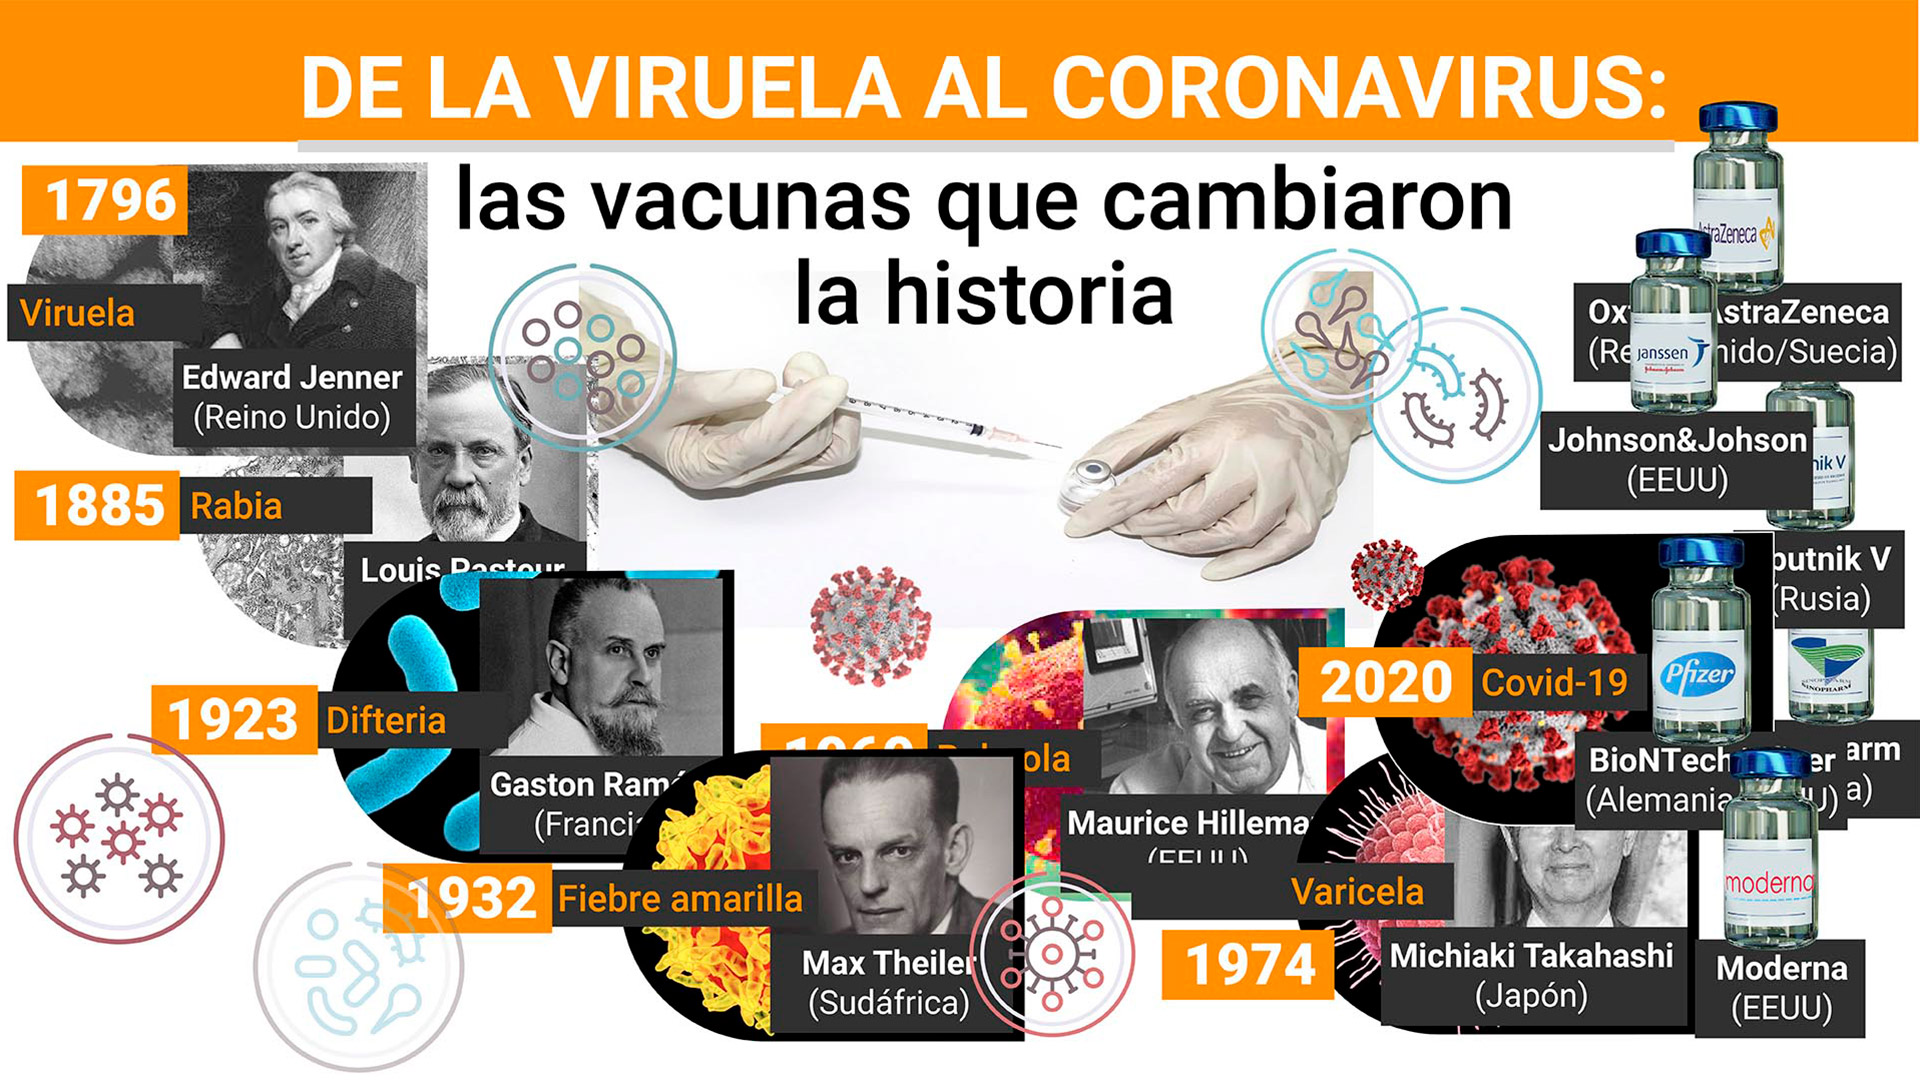
\includegraphics[width=0.7\textwidth]{img/vacunación.jpg}
        \caption{Historia de la vacunación, desde el inicio a la actualidad}
        \label{fig:vacunación}
        \vspace{0.5cm} % Ajusta el espacio vertical entre la imagen y el texto
    \end{figure}



\subsection{Impacto y desafíos actuales}
A pesar del impacto positivo y ampliamente documentado de la vacunación, según \cite{lindstrand2021world}persisten diversos desafíos que afectan su implementación y sostenibilidad a nivel global:
\begin{itemize}
    \item \textbf{Hesitación vacunal y desconfianza}: la desinformación, las creencias en métodos alternativos o "naturales" y la falta de confianza en los sistemas sanitarios generan una baja aceptación de las vacunas en ciertos grupos. 
    \item \textbf{Desigualdades en el acceso}: en regiones de bajos ingresos, existen barreras económicas, logísticas y estructurales que dificultan la distribución equitativa de vacunas. Iniciativas como \textbf{\textit{GAVI}}\footnote{Global Alliance for Vaccines and Immunisation, consorcio internacional compuesto por diversas entidades objetivo es facilitar el acceso a vacunas en países menos desarrollados}, han mejorado la situación, pero aún persisten importantes brechas.
    \item \textbf{Infraestructura limitada}: los sistemas de salud en países de ingresos bajos suelen carecer del personal capacitado, recursos financieros y logística necesarios para mantener programas de vacunación sostenibles.
    \item \textbf{Impacto de la pandemia de COVID-19}: la crisis sanitaria interrumpió programas de vacunación rutinaria, reduciendo las tasas de cobertura y aumentando la exposición a enfermedades prevenibles.
    \item \textbf{Resurgimiento de enfermedades}: La disminución en la cobertura vacunal ha provocado brotes recientes de enfermedades. La OMS insiste en la necesidad de mantener altas tasas de cobertura para prevenir estas situaciones.
\end{itemize}



\section{SIDA/VIH}
Según \cite{sudharshan2008introduction} el síndrome de inmunodeficiencia adquirida (SIDA)  es una enfermedad causada por la infección del virus de la inmunodeficiencia humana (VIH). El VIH es un retrovirus que ataca y destruye las células CD4+T, esenciales para el sistema inmunológico, lo que provoca una inmunodeficiencia progresiva. Las personas infectadas se vuelven más susceptibles a infecciones y ciertos tipos de cáncer. La estructura del VIH se observa en la figura \ref{fig:vih estructura}\footnote{Obtenida de \cite{infosida_vih}}

\begin{figure}[H]
    \centering
    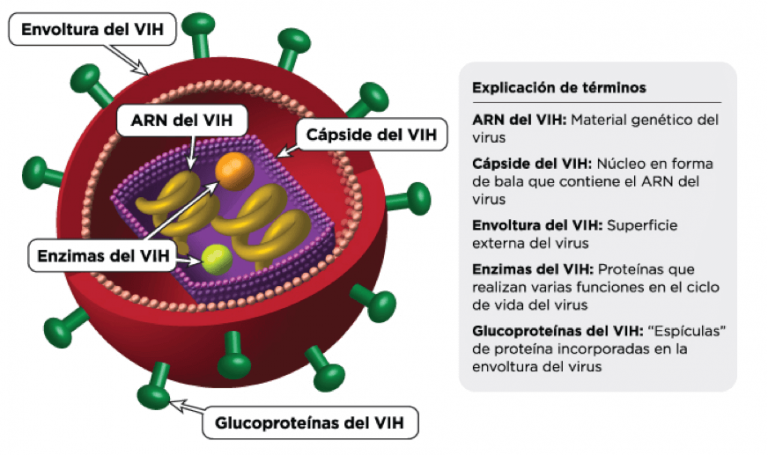
\includegraphics[width=0.7\textwidth]{img/vih_estructura.png}
    \caption{Estrucutura del virus de la inmunodeficiencia humana (VIH)}
    \label{fig:vih estructura}
    \vspace{0.5cm} % Ajusta el espacio vertical entre la imagen y el texto
\end{figure}

\subsection{Vías de transmisión}
El VIH se transmite a través de varias vías bien definidas, como se explica en \cite{shaw2012hiv}:
\begin{itemize}
    \item Contacto sexual: principal forma de transmisión. Ocurre en relaciones sexuales vaginales, anales y orales sin protección, mediante fluidos infectados.
    \item Uso compartido de agujas: frecuente entre personas usuarias de drogas intravenosas. Vía de alto riesgo por la introducción directa del virus en la sangre.
    \item Transfusiones de sangre y productos sanguíneos: aunque posible, su riesgo es mínimo en países donde se realizan pruebas rigurosas en bancos de sangre.
    \item Transmisión madre-hijo: puede ocurrir durante el embarazo, parto o lactancia. El uso de TAR\footnote{Terapia Antirretroviral} y cesáreas programadas reduce el riesgo.
    \item Trasplantes de órganos: es raro debido a los controles exhaustivos.
    \item Exposición ocupacional: riesgo bajo en profesionales de la salud si se siguen las precauciones adecuadas.
\end{itemize}

\subsection{Diagnóstico}
El diagnóstico se basa en:
\begin{enumerate}
    \item Inmunoensayo combinado Ag/Ab: detecta anticuerpos contra VIH-1/VIH-2 y antígeno p24. Puede identificar la infección 2–3 semanas después de la exposición \cite{workowski2021sexually}.
    \item Prueba de diferenciación de anticuerpos: permite distinguir entre VIH-1 y VIH-2.
    \item Prueba de amplificación de ácidos nucleicos (NAAT): se emplea si hay resultados indeterminados. Confirma infecciones agudas por VIH-1 \cite{saag2021hiv}.
    \item Pruebas rápidas: Ofrecen resultados preliminares en menos de 20 minutos. Se deben confirmar con pruebas de laboratorio.
\end{enumerate}

\subsection{Tratamiento}
El tratamiento se basa en TAR \cite{heendeniya2019antiretroviral}, que ha convertido al VIH en una enfermedad crónica controlable.

\textbf{Opciones terapéuticas}. Según \cite{sivanandy2023efficacy} los INSTI\footnote{Inhibidores de la transferencia de cadena de la integrasa} constituyen la primera línea de tratamiento, generalmente combinados con tenofovir. Además, se utilizan terapias de acción prolongada.

\textbf{Consideraciones clínicas}. Según \cite{saag2021hiv} Entre los efectos secundarios se incluyen náuseas, cefaleas, acidosis láctica y hepatomegalia con esteatosis. Es fundamental ajustar el tratamiento considerando la función renal y hepática del paciente, así como posibles interacciones medicamentosas.

\textbf{Impacto psicosocial}. El estigma asociado al VIH puede afectar negativamente la adherencia al tratamiento y la calidad de vida de los pacientes. El apoyo psicológico y social resulta esencial para mejorar su bienestar general \cite{cihlar2016current}.

\subsection{Estrategias de prevención}
La prevención del VIH/SIDA \cite{chan2012biomedical} combina medidas farmacológicas, no farmacológicas y de salud pública, como se observa .

\textbf{Enfoques farmacológicos}.
La PrEP\footnote{Profilaxis preexposición} consiste en el uso diario de antirretrovirales en personas con alto riesgo de contraer el virus. La PEP\footnote{Profilaxis postexposición} implica la administración inmediata de antirretrovirales tras una posible exposición. Además, el TasP\footnote{Tratamiento como prevención} se basa en que las personas con carga viral indetectable no transmiten el virus (indetectable = intransmisible).

\textbf{Enfoques no farmacológicos}.
Se encuentra el uso de preservativos como barrera física, la circuncisión masculina que reduce el riesgo de infección, la educación para promover prácticas sexuales seguras, y los programas de intercambio de agujas que disminuyen la transmisión entre usuarios de drogas intravenosas.

\textbf{Medidas de salud pública}.
Incluyen el diagnóstico temprano del VIH para iniciar el tratamiento oportuno, la prevención de la transmisión de madre a hijo mediante intervenciones médicas, y las intervenciones estructurales destinadas a reducir desigualdades sociales.

\subsection{Progresión clínica}
Tras la infección inicial, se observan tres fases:
\begin{enumerate}
    \item \textbf{Fase aguda}: síntomas similares a los de una gripe.
    \item \textbf{Fase de latencia clínica}: puede durar años; el paciente es asintomático mientras el virus se replica en niveles bajos.
    \item \textbf{Progresión a SIDA}: ocurre como se explica en \cite{okoye2013cd}cuando el recuento de CD4+ cae por debajo de 200 células/µL o aparecen infecciones oportunistas como sarcoma de Kaposi o candidiasis esofágica.
\end{enumerate}
La media del tiempo entre la infección y el desarrollo de SIDA en ausencia de tratamiento es de 8 a 10 años. Factores como la carga viral, coinfecciones o la respuesta inmune individual influyen en la progresión \cite{hoover1992progression}.

\subsection{Evolución e impacto}
Desde los años 80, el impacto del SIDA ha cambiado significativamente gracias al desarrollo de TARGA\footnote{Terapia antirretroviral de gran actividad}. La incidencia de enfermedades oportunistas se redujo drásticamente, pasando de 30.7 a 2.5 casos por cada 100 años-paciente entre 1994 y 1998, según el estudio EuroSIDA\footnote{estudio observacional de cohortes prospectivo que sigue a personas con VIH} \cite{mocroft2000aids}. Además, se ha observado un aumento en el recuento de células CD4+ en los diagnósticos recientes, lo que indica un mejor manejo clínico de la enfermedad. Sin embargo, el impacto del SIDA no ha sido uniforme, ha habido un aumento de infecciones en mujeres, jóvenes y minorías. Los avances en pruebas diagnósticas, como las pruebas rápidas orales, han facilitado la detección temprana del VIH, aunque persisten desafíos importantes, como el diagnóstico tardío \cite{san2003incidence}.
En la figura \ref{fig:evolución vih}\footnote{Obtenido en \cite{madrid_salud_poblacion}} se puede observar la evolución en la Comunidad de Madrid 

\begin{figure}[H]
    \centering
    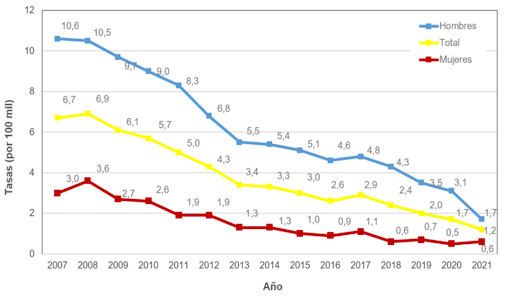
\includegraphics[width=0.7\textwidth]{img/evolucionVIH.png}
    \caption{Evolución VIH en la Comunidad de Madrid de 2007 a 2021}
    \label{fig:evolución vih}
    \vspace{0.5cm} % Ajusta el espacio vertical entre la imagen y el texto
\end{figure}

\section{Gonorrea}
La gonorrea según \cite{unemo2019gonorrhoea} es una infección o enfermedad de transmisión sexual causada por la bacteria \textit{Neisseria gonorrhoeae}, se puede observar en la figura \ref{fig:Neisseria gonorrhoeae}\footnote{Obtenida de \cite{vircell_gonorrhoeae}}. Puede afectar el tracto urogenital, recto o faringe. De las más comunes a nivel mundial, con una incidencia anual estimada de 86.9 millones de casos en adultos.

\begin{figure}[H]
    \centering
    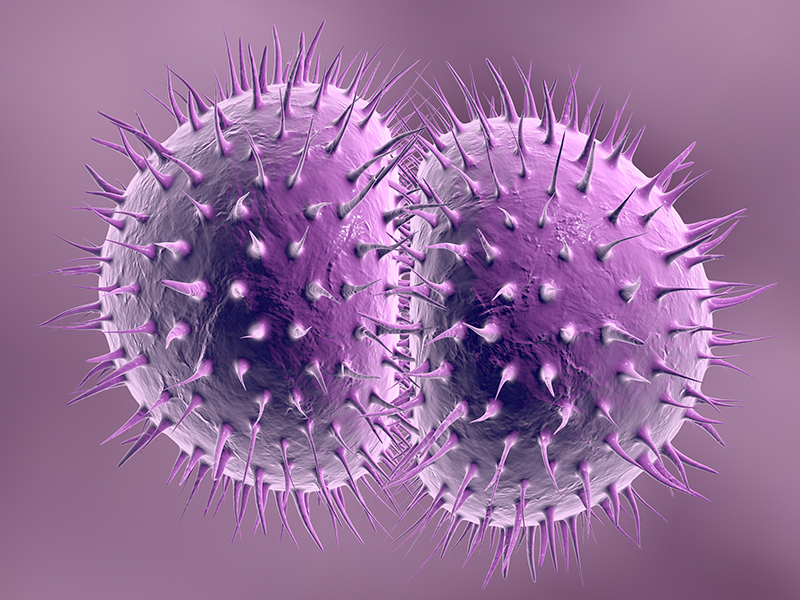
\includegraphics[width=0.7\textwidth]{img/NeisseriaGonorrhoeae.jpg}
    \caption{Forma de la bacetria Neisseria gonorrhoeae}
    \label{fig:Neisseria gonorrhoeae}
    \vspace{0.5cm} % Ajusta el espacio vertical entre la imagen y el texto
\end{figure}


\subsection{Vías de transmisión}
Se transmite principalmente a través del contacto sexual sin protección \cite{workowski2021sexually}. Durante las relaciones sexuales vaginales, puede infectar el tracto genital tanto en hombres como en mujeres. En las relaciones anales, la infección puede afectar el recto. Asimismo, durante el sexo oral sin protección, puede colonizar la faringe.

Otra vía de transmisión es la perinatal, en la cual una madre infectada puede transmitir la bacteria a su bebé durante el parto. También se ha documentado la posibilidad de transmisión al utilizar saliva como lubricante, especialmente entre hombres que tienen sexo con hombres. Además, aunque de forma menos común, existe evidencia limitada que sugiere que la gonorrea orofaríngea podría transmitirse a través del beso profundo.

\subsection{Diagnóstico}
El diagnóstico de la gonorrea debe considerar las posibles infecciones en el tracto urogenital, recto y faringe. Los métodos principales incluyen  NAAT\footnote{Pruebas de amplificación de ácidos nucleicos}, cultivo bacteriano y tinción de Gram incluidos en \cite{adamson2022diagnostic}.

Las NAAT son el estándar de oro (gold standard) debido a su alta sensibilidad y especificidad. Permiten el uso de diferentes tipos de muestras. Además, ofrecen la ventaja de facilitar el autodiagnóstico mediante muestras autocolectadas por los pacientes.

El cultivo bacteriano, aunque menos sensible que las NAAT, sigue siendo fundamental para la detección de cepas resistentes a los antimicrobianos. Requiere muestras como las uretrales, endocervicales, rectales, faríngeas o conjuntivales, y es útil para realizar pruebas de susceptibilidad en casos de fracaso del tratamiento.

La tinción de Gram puede ser diagnóstica en hombres sintomáticos cuando se observan diplococos gramnegativos intracelulares en secreciones uretrales. Sin embargo, su sensibilidad es menor en mujeres y en sitios extragenitales, por lo que no se recomienda como única prueba diagnóstica en estos casos.

La combinación de estos métodos permite un diagnóstico oportuno y efectivo, lo que es clave para el tratamiento adecuado y la prevención de complicaciones y nuevas transmisiones.

\subsection{Tratamiento}
La gonorrea ha desarrollado resistencia a múltiples antibióticos a lo largo del tiempo. Actualmente, el tratamiento recomendado según \cite{cyr2020update} es una dosis única de ceftriaxona, con la posible adición de doxiciclina si no se ha descartado coinfección por Chlamydia trachomatis.

Debido al aumento de la resistencia a medicamentos como la azitromicina \cite{unemo2019antimicrobial}, es fundamental la vigilancia continua de la eficacia de los tratamientos. En caso de sospecha de fallo terapéutico, se recomienda realizar pruebas de susceptibilidad y confirmar la curación, especialmente en infecciones faríngeas. La investigación actual se centra en el desarrollo de nuevos antimicrobianos y vacunas para combatir la resistencia emergente.

\subsection{Prevención}
Estrategias recomendadas incluidas en \cite{mayor2012diagnosis} son:
\begin{itemize}
    \item Uso correcto de preservativos.
    \item Educación y consejería sobre prácticas sexuales seguras y reducción de riesgos.
    \item Detección y tratamiento de parejas sexuales para evitar reinfecciones y transmisión. 
    \item Cribado regular.
    \item Promoción de salud pública, acceso a servicios, reducción del estigma y políticas efectivas.
\end{itemize}

\subsection{Clínica y complicaciones}
Los síntomas de la gonorrea varían según el sexo \cite{unemo2019gonorrhoea}. En los hombres, se manifiesta comúnmente como uretritis con disuria y secreción purulenta. En las mujeres, muchas veces es asintomática, aunque puede presentarse como cervicitis con secreción mucopurulenta y dolor pélvico.

Las complicaciones también difieren. En las mujeres, puede derivar en enfermedad inflamatoria pélvica, infertilidad, embarazo ectópico y dolor crónico. En los hombres, la principal complicación es la epididimitis, que también puede conllevar infertilidad. En ambos sexos, existe el riesgo de desarrollar una infección gonocócica diseminada.

Las infecciones extragenitales incluyen proctitis, faringitis que suele ser asintomática y conjuntivitis neonatal cuando ocurre transmisión perinatal.

Desde el punto de vista de la salud pública, la gonorrea incrementa el riesgo de transmisión del VIH. Además, la creciente resistencia a los antimicrobianos representa un desafío significativo para su control y tratamiento.

\subsection{Historia y evolución}
La gonorrea ha sido una infección de transmisión sexual prevalente durante miles de años. Desde la introducción de los antibióticos, \textit{Neisseria gonorrhoeae} ha desarrollado resistencia progresiva a cada clase utilizada. Primero se observó con las sulfonamidas y penicilinas en las décadas de 1940 y 1950. Posteriormente, surgió resistencia a las tetraciclinas y macrólidos, y más tarde a las fluoroquinolonas durante las décadas de 1980 y 1990.

En la actualidad, la terapia recomendada que anteriormente incluía el uso dual de ceftriaxona y azitromicina también enfrenta un aumento preocupante en la resistencia, con casos reportados de cepas resistentes a ambos antibióticos. Un ejemplo de ello es el clon FC428, resistente a la ceftriaxona, que se ha diseminado a nivel mundial desde 2017 \cite{golparian2020genomic}.

Esta evolución subraya la necesidad urgente de desarrollar nuevas estrategias terapéuticas y medidas efectivas de prevención para controlar la propagación de esta infección \cite{lin2021epidemiology}.
En la figura \ref{fig:evolución gonorrea} obtenida de \cite{isanidad2023}, se observa como ha evolucionado la gonorrea en España, donde se ve que los casos han aumentado, una causa puede ser la resitencia a los antibióticos.

\begin{figure}[H]
    \centering
    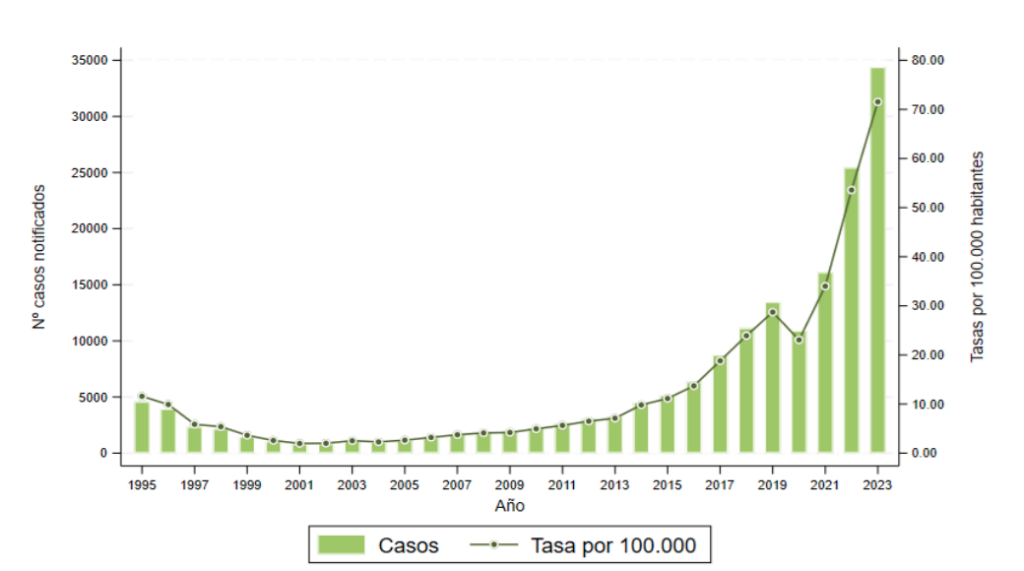
\includegraphics[width=0.7\textwidth]{img/incidenciagonorrea.png}
    \caption{Evolución gonorrea en España de 1995 a 2023}
    \label{fig:evolución gonorrea}
    \vspace{0.5cm} % Ajusta el espacio vertical entre la imagen y el texto
\end{figure}


\section{Sarampión}
El sarampión según \cite{workowski2021sexually}es una enfermedad vírica altamente contagiosa, causada por el MeV\footnote{Virus del sarampión}. Antes de la introducción de la vacuna, prácticamente todos los niños la contraían durante la infancia. La transmisión se produce por vía respiratoria. Se caracteriza por fiebre, tos, coriza, conjuntivitis y exantema maculopapular, se observa en la figura \ref{fig:sarampión}\footnote{Obtenida de \cite{tododiagnostico2020sarampion}}.

\begin{figure}[H]
        \centering
        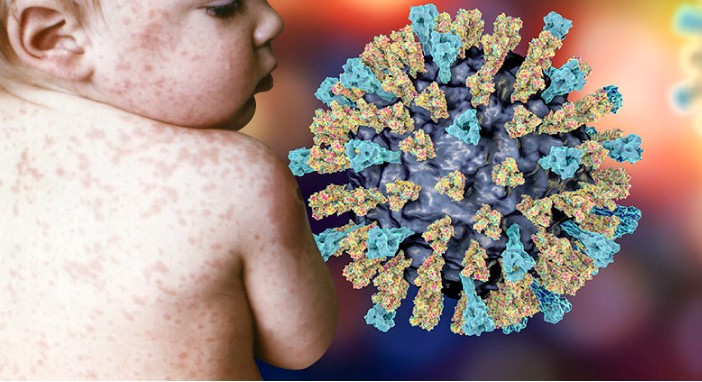
\includegraphics[width=0.7\textwidth]{img/sarampion.jpg}
        \caption{Representación del virus del sarampión (MeV) junto a la manifestación clínica típica de la enfermedad exantema maculopapular}
        \label{fig:sarampión}
        \vspace{0.5cm} % Ajusta el espacio vertical entre la imagen y el texto
\end{figure}

\subsection{Vías de transmisión}
El sarampión se transmite de persona a persona a través de gotitas respiratorias y por vía aérea mediante núcleos de gotitas aerosolizadas. Las personas infectadas son contagiosas desde cuatro días antes hasta cuatro días después de la aparición del exantema. Es una de las enfermedades víricas más contagiosas conocidas, con tasas de ataque iguales o superiores al 90\% entre contactos susceptibles. Los seres humanos son el único huésped natural del virus del sarampión, lo que hace factible su erradicación a nivel global \cite{moss2017measles}.

\subsection{Diagnóstico}
El diagnóstico se basa \cite{baeten2012antiretroviral} en una combinación de criterios clínicos y confirmación mediante pruebas de laboratorio.

\textbf{Presentación clínica}: el sarampión se caracteriza por fiebre, exantema maculopapular y al menos uno de los tres signos clásicos: tos, coriza y conjuntivitis. Un hallazgo clínico distintivo son las manchas de Koplik, pequeñas lesiones blanquecinas en la mucosa bucal que suelen aparecer antes del exantema.

\textbf{Confirmación de laboratorio}:
\begin{enumerate}
    \item Detección de anticuerpos IgM específicos contra el virus del sarampión: método más común y se realiza mediante ELISA\footnote{Ensayo de inmunoadsorción ligado a enzima}. Tiene una sensibilidad del 83–89\% y una especificidad del 95–99\%. No obstante, los anticuerpos IgM pueden no ser detectables en alrededor del 25\% de los casos durante las primeras 72 horas tras la aparición del exantema, aunque casi siempre están presentes después de 4 días.
    \item RT-PCR\footnote{PCR de transcripción inversa} para la detección de ARN del virus del sarampión: permite identificar material genético del virus en muestras de orina, sangre, secreciones nasofaríngeas o fluidos orales. Presenta una sensibilidad del 94\% y una especificidad del 99\%. La RT-PCR es útil en las etapas tempranas de la enfermedad, antes de que se desarrollen los anticuerpos IgM. Además, permite la genotipificación del virus, lo que facilita el seguimiento epidemiológico de su propagación.
    \item Seroconversión de IgG: la confirmación mediante seroconversión o un incremento de cuatro veces en los títulos de IgG entre la fase aguda y la fase convaleciente también es válida, aunque se utiliza con menor frecuencia debido a la disponibilidad limitada de pruebas cuantitativas de IgG en muchos laboratorios clínicos locales.
\end{enumerate}

\subsection{Tratamiento}
Las intervenciones terapéuticas clave en el artúclo \cite{graber2020update} son las siguientes.

\textbf{Terapia de soporte}.
Incluye una adecuada hidratación y el control de los síntomas como la fiebre y la tos, a través del uso de antipiréticos y otros cuidados generales.

\textbf{Suplementación con vitamina A}.
La OMS recomienda la administración de vitamina A en todos los casos de sarampión agudo en niños, independientemente del país de residencia, con el objetivo de reducir el riesgo de complicaciones graves.
Consiste en dosis orales administradas una vez al día durante dos días. En casos de deficiencia clínica de vitamina A, se recomienda una tercera dosis.

\textbf{Tratamiento de infecciones bacterianas secundarias}.
El sarampión puede predisponer a infecciones bacterianas como la neumonía o la otitis media. Se deben administrar antibióticos adecuados, según la infección y la susceptibilidad del paciente.

\textbf{Aislamiento y prevención de la transmisión}.
Los pacientes deben ser aislados para evitar la transmisión del virus. Se deben implementar medidas de control de infecciones, como el uso de mascarillas.

\subsection{Prevención}
Puede prevenirse mediante la vacunación. Se administra en formulaciones combinadas, como la SRP (sarampión, paperas y rubéola) se muestra en la figura \ref{fig:vacuna sarampión}\footnote{Obtenida de \cite{aarp_sarampion_2019}} o la SRPV (que también incluye varicela), ha demostrado ser segura y efectiva.

\begin{figure}[H]
        \centering
        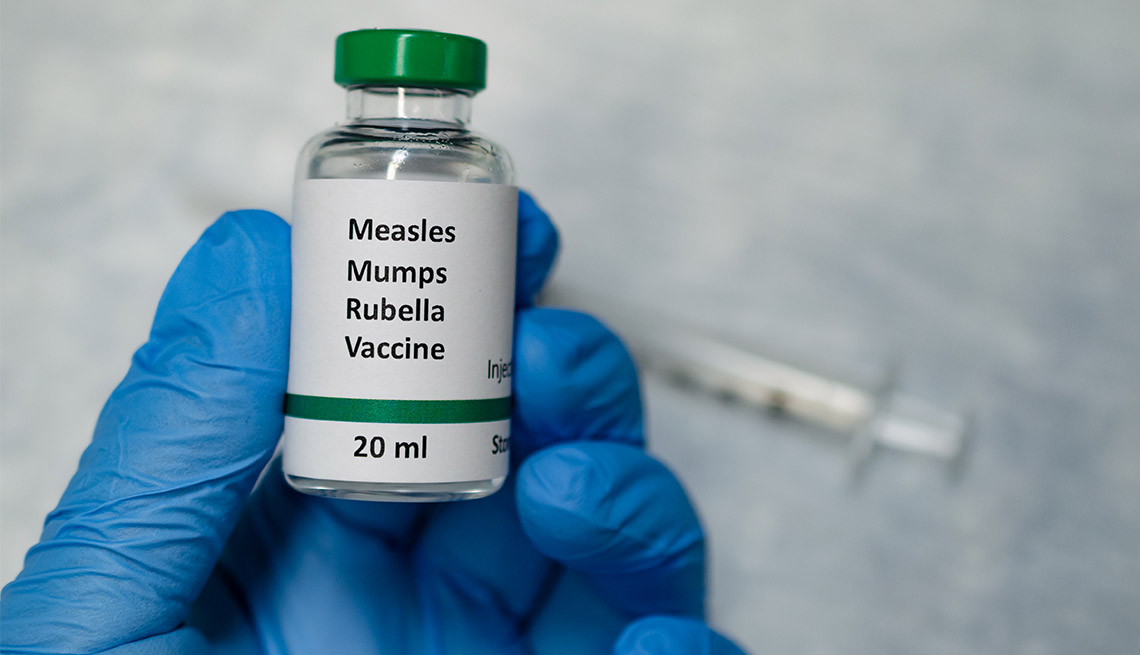
\includegraphics[width=0.7\textwidth]{img/vacunaMMR.jpg}
        \caption{Vacuna triple de sarampión, paperas y rubeola, siglas inglés MMV}
        \label{fig:vacuna sarampión}
        \vspace{0.5cm} % Ajusta el espacio vertical entre la imagen y el texto
\end{figure}

Se recomienda la administración de dos dosis de la vacuna SRP: la primera entre los 12 y 15 meses de edad y la segunda entre los 4 y 6 años \cite{gastanaduy2021measles}. 

Debe priorizarse la vacunación en grupos con mayor riesgo de exposición, como estudiantes, personal sanitario o viajeros internacionales.

En personas susceptibles, la administración de la vacuna dentro de las 72 horas tras la exposición puede prevenir o reducir la gravedad del sarampión. Alternativamente, la inmunoglobulina humana puede administrarse hasta 6 días después, especialmente en lactantes, embarazadas no inmunizadas y personas inmunodeprimidas.

Dado que la inmunoglobulina proporciona una inmunidad temporal, se recomienda completar la vacunación con SRP tras un intervalo mínimo de 6 meses (intramuscular) u 8 meses (intravenosa). Mantener una cobertura vacunal igual o superior a 95\% es fundamental para evitar brotes y avanzar hacia la eliminación del sarampión.

\subsection{Progeresión clínica y complicaciones}
Sigue una evolución clínica característica, dividida en varias fases como se explica en \cite{cdc_measles}:
\begin{enumerate}
    \item \textbf{Fase prodrómica}: dura de 2 a 4 días e incluye fiebre alta, tos, coriza y conjuntivitis. Son típicas las manchas de Koplik en la mucosa bucal.
    \item \textbf{Fase exantemática}: alrededor de 14 días tras la exposición, aparece un exantema maculopapular que comienza en la cara y se extiende al tronco y extremidades, persistiendo entre 4 y 7 días.
    \item \textbf{Recuperación}: en casos no complicados, el exantema desaparece en orden inverso a su aparición y la recuperación completa se da en torno a una semana después.
\end{enumerate}

Puede ocasionar complicaciones graves, especialmente en niños pequeños, adultos mayores, embarazadas, personas desnutridas o inmunocomprometidas. Las más frecuentes son: otitis media, neumonía, diarrea, encefalitis o SSPE \footnote{Panencefalitis esclerosante subaguda}.

\subsection{Impacto histórico y situación actual}
El sarampión ha tenido un impacto significativo en la salud pública mundial. Antes de la introducción de la vacuna, era una enfermedad endémica que afectaba a la mayoría de los niños y causaba millones de muertes al año. Las epidemias eran frecuentes.

Con la llegada de la vacunación, la incidencia del sarampión disminuyó de forma drástica. Entre 2000 y 2017, los casos a nivel global se redujeron en un 83\%, y las muertes anuales pasaron de 545 mil a 109 mil como se destaca en \cite{shanks2014measles}. 

No obstante, sigue siendo una causa importante de mortalidad infantil en regiones con baja cobertura vacunal y sistemas de salud frágiles. Además, la reaparición de brotes en algunos países se ha asociado a la desinformación sobre la vacuna y la disminución en las tasas de vacunación. La interrupción de las campañas de inmunización durante la pandemia de COVID-19 ha agravado este riesgo \cite{fischer2016zinc}.

En la figura \ref{fig:evolución sarampión}, tomada de \cite{ahumada2015modelos}, se muestra un ejemplo del caso de Chile, donde se observa la evolución del sarampión entre los años 1939 y 2014. La figura evidencia una notable disminución en la incidencia de la enfermedad a partir de la introducción de la vacuna, con una caída aún más significativa tras la implementación de campañas de vacunación, hasta alcanzar la eliminación de casos reportados.

\begin{figure}[H]
        \centering
        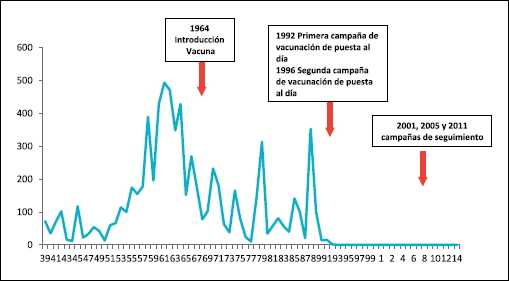
\includegraphics[width=0.7\textwidth]{img/evolucionSarampion.jpg}
        \caption{Tasa de incidencia de sarampión en Chile 1939-2014, asociado a inclusión de la vacuna y campañas de vacunación.}
        \label{fig:evolución sarampión}
        \vspace{0.5cm} % Ajusta el espacio vertical entre la imagen y el texto
\end{figure}

\section{COVID-19}
El COVID-19\footnote{Enfermedad por coronavirus} es causada por el virus SARS-CoV-2 figura \ref{fig:covid estructura}\footnote{Obtenida de \cite{medlineplus_sarscov2}}, altamente transmisible que surgió a finales de 2019 en Wuhan, China. Su transmisión se produce a través de gotículas respiratorias generadas al hablar, toser o estornudar, durante el contacto cercano. No obstante, también puede propagarse mediante aerosoles en espacios cerrados, así como por contacto con superficies contaminadas.

\begin{figure}[H]
        \centering
        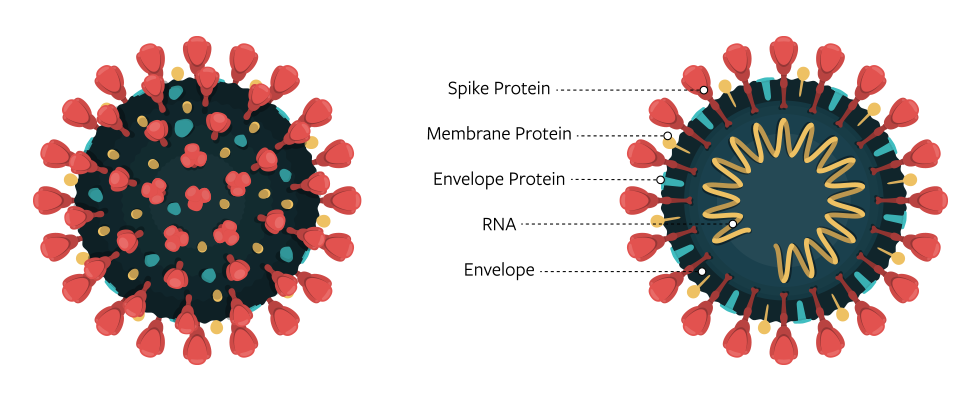
\includegraphics[width=0.7\textwidth]{img/estructuracovid.png}
        \caption{Estructura del virus SARS-CoV-2 (COVID-19).}
        \label{fig:covid estructura}
        \vspace{0.5cm} % Ajusta el espacio vertical entre la imagen y el texto
\end{figure}

\subsection{Vías de transmsión}
Se transmite principalmente mediante partículas respiratorias emitidas al toser, estornudar, hablar o respirar. Según \cite{wiersinga2020covid19}existen varios mecanismos de transmisión:
\begin{itemize}
    \item Gotas respiratorias: partículas de mayor tamaño que se depositan rápidamente, facilitando la transmisión a corta distancia.
    \item Aerosoles: partículas más pequeñas que pueden permanecer suspendidas en el aire, en espacios cerrados y mal ventilados, permitiendo la transmisión a mayor distancia.
    \item Fómites: aunque el virus puede sobrevivir en superficies inanimadas durante horas o días, forma de contagio menos frecuente.
    \item Transmisión asintomática: individuos sin síntomas pueden transmitir el virus, especialmente en las fases presintomáticas, contribuye a su propagación.
\end{itemize}

\subsection{Diagnóstico}
Se fundamenta principalmente \cite{ko2022covid} en la detección del ARN del SARS-CoV-2 mediante pruebas moleculares, especialmente la RT-PCR, considerada el método de referencia por su alta sensibilidad y especificidad.

\textbf{RT-PCR}: se realiza sobre muestras respiratorias y permite detectar el virus en fases tempranas, se observa en la figura \ref{fig:PCR}\footnote{\cite{comunidadmadrid2020pcr}}.

\begin{figure}[H]
        \centering
        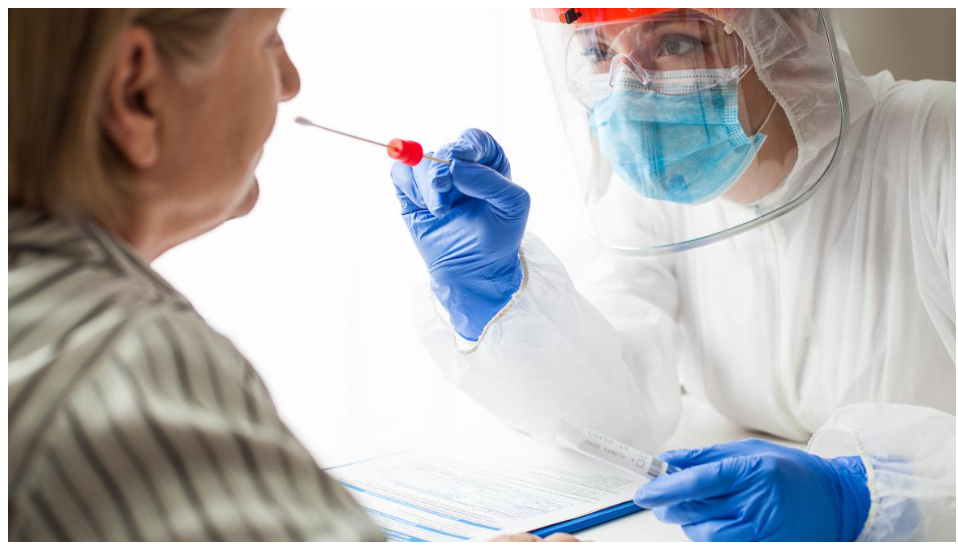
\includegraphics[width=0.7\textwidth]{img/pcr.png}
        \caption{Toma de muestra nasofaríngea para la realización de una prueba PCR con el fin de detectar la presencia del virus SARS-CoV-2 (COVID-19).}
        \label{fig:PCR}
        \vspace{0.5cm} % Ajusta el espacio vertical entre la imagen y el texto
\end{figure}

\textbf{Pruebas de antígenos}: aunque menos sensibles, ofrecen resultados rápidos y son útiles en entornos donde se requiere diagnóstico inmediato, se muestra en la figura \ref{fig:antigenos}\footnote{Obtenida de \cite{ceydes_antigeno}}.

\begin{figure}[H]
        \centering
        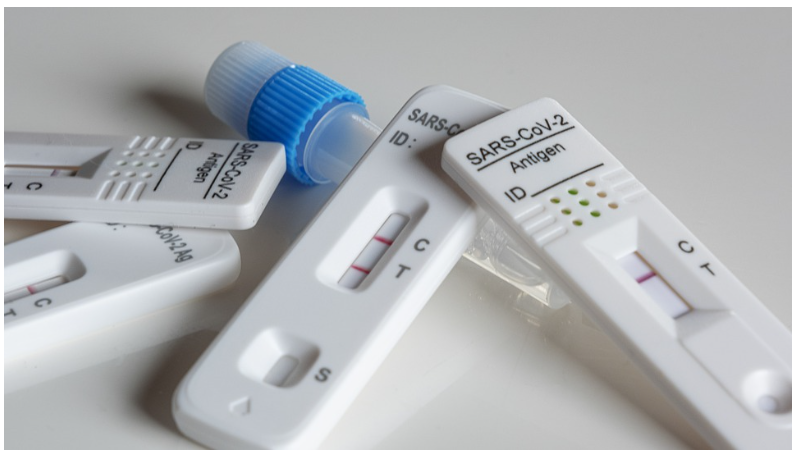
\includegraphics[width=0.7\textwidth]{img/prueba antigenos.png}
        \caption{Test de antígenos para SARS-CoV-2. Resultado positivo (se observan líneas en la zonas de control (C) y test (T)) y negativo (se observa solo línea en control (C)).}
        \label{fig:antigenos}
        \vspace{0.5cm} % Ajusta el espacio vertical entre la imagen y el texto
\end{figure}

\textbf{Pruebas serológicas}: detectan anticuerpos y son útiles para estudios epidemiológicos, pero no para el diagnóstico en fases agudas.

\subsection{Tratamiento}
Varía según la gravedad del cuadro clínico.

En casos leves o moderados, se basa en medidas como el reposo, la hidratación, el control de la fiebre y el dolor, y el seguimiento domiciliario. En pacientes con factores de riesgo, se recomienda un monitoreo más estrecho para detectar complicaciones \cite{qaseem2023outpatient}.

En casos graves, requieren hospitalización y soporte respiratorio, incluyendo oxigenoterapia. Se emplean tratamientos específicos para reducir la inflamación, prevenir complicaciones como la trombosis, y mejorar la respuesta inmunitaria. En algunos casos, es necesario el ingreso en UCI y el uso de ventilación mecánica \cite{wiersinga2020pathophysiology}.

\subsection{Medidas de prevención}
Las principales medidas para prevenir el COVID-19 incluidas en \cite{hutchins2020covid}:
\begin{itemize}
    \item Vacunación, herramienta más eficaz para reducir la gravedad de la enfermedad. Se recomienda para todas las personas mayores de 6 meses.
    \item Uso de mascarilla, útil en espacios cerrados, especialmente en situaciones de alta transmisión.
    \item Distanciamiento físico y ventilación, mantener una distancia adecuada y mejorar la ventilación en interiores.
    \item Higiene de manos: lavarse frecuentemente con agua y jabón o usar gel hidroalcohólico.
    \item Recomendaciones para personas de alto riesgo, además de las medidas generales, deben mantenerse al día con las dosis de refuerzo, considerar el uso de antivirales tras una exposición y monitorizar su estado de salud en casa. En caso de infección, deben seguir las recomendaciones de aislamiento.
\end{itemize} 
Estas estrategias, combinadas, son clave para reducir la transmisión y proteger a la población más vulnerable.

\subsection{Progresión clínica}
La evolución varía desde formas asintomáticas hasta cuadros críticos. Generalmente se explica en \cite{cdc_covid19_yellowbook} que sigue estas fases:

\begin{enumerate}
    \item Incubación e inicio: el periodo de incubación es de 2 a 14 días. Los síntomas iniciales incluyen fiebre, tos, malestar, dolor de garganta, mialgias, y en algunos casos síntomas gastrointestinales. La pérdida del olfato y gusto es frecuente.
    \item Fase prodrómica (1ª semana): aparecen síntomas respiratorios leves o moderados. Puede observarse neumonía incipiente y alteraciones leves en marcadores inflamatorios.
    \item Fase aguda (2ª semana): se intensifican los síntomas, especialmente la disnea. Pueden aparecer complicaciones como neumonía grave, daño cardíaco o trastornos de coagulación. Los marcadores inflamatorios y hematológicos alcanzan sus niveles más alterados.
    \item Fase de remisión (3ª semana): los síntomas comienzan a mejorar, aunque la inflamación puede persistir.
    \item Convalecencia, la recuperación puede tardar semanas, dependiendo de la gravedad del cuadro.
\end{enumerate}

Factores de riesgo: edad avanzada, enfermedades crónicas (cardiovasculares, pulmonares, diabetes, obesidad) y alteraciones inmunológicas aumentan el riesgo de enfermedad grave.

Hallazgos clínicos, en casos graves, se observan linfopenia y elevación de marcadores como dímero D, PCR y ferritina. Las imágenes pulmonares suelen mostrar opacidades en vidrio esmerilado.

\subsection{Impacto de la pandemia del COVID-19}
Ha tenido consecuencias profundas a nivel global, afectando múltiples aspectos de la sociedad. 

Salud pública. Con más de 774 millones de casos y 7 millones de muertes hasta febrero de 2024, la incidencia se puede observar en la figura \ref{fig:muertes covid}\footnote{Obtenida de \cite{elpais_covidmap}}, la pandemia desbordó los sistemas de salud, generando escasez de recursos y personal médico, especialmente en poblaciones vulnerables.
\begin{figure}[H]
        \centering
        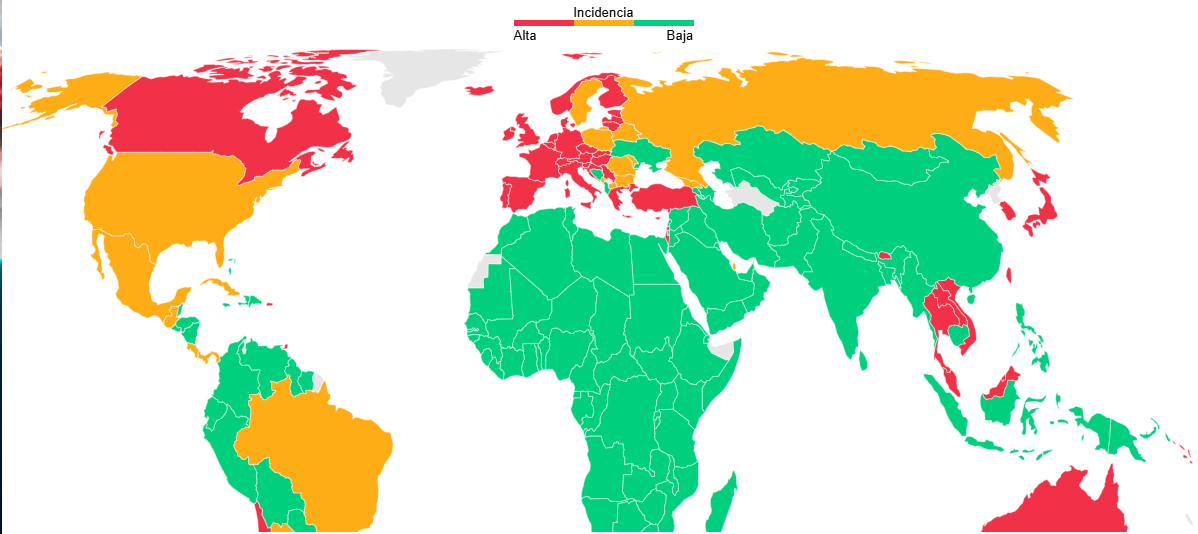
\includegraphics[width=0.7\textwidth]{img/covid_muertes.png}
        \caption{Distribución global de la incidencia de muertes hasta el 2 de febrero de 2025, categorizada por intensidad: baja (verde), media (naranja) y alta (rojo).}
        \label{fig:muertes covid}
        \vspace{0.5cm} % Ajusta el espacio vertical entre la imagen y el texto
\end{figure}
\begin{itemize}
    \item Economía. Las medidas de confinamiento y el cierre de actividades causaron una fuerte recesión global, afectando gravemente sectores como el turismo, la hostelería y el comercio, y acentuando las desigualdades económicas.
    \item Vida social y salud mental. El aislamiento y la incertidumbre aumentaron los niveles de ansiedad, depresión y otros trastornos mentales, al tiempo que se intensificaron el estigma y la discriminación hacia ciertos grupos.
    \item Educación. El cierre de centros educativos forzó una transición abrupta a la educación en línea, revelando y ampliando las brechas digitales, especialmente en estudiantes de bajos recursos.
    \item Medio ambiente. La reducción de la actividad humana durante los confinamientos produjo efectos positivos temporales, como la disminución de emisiones contaminantes y la mejora en la calidad del aire.
\end{itemize}

La pandemia evidenció vulnerabilidades globales y la necesidad de fortalecer sistemas sanitarios, reducir desigualdades y prepararse mejor para futuras emergencias \cite{miyah2022covid}.

\section{Ingeniería de control}
La ingeniería de control es una disciplina de la ingeniería que se encarga del análisis y diseño de sistemas capaces de autorregularse para alcanzar un comportamiento deseado. Su objetivo es influir sobre el comportamiento dinámico de un sistema, de modo que, ante ciertas entradas o perturbaciones, se obtenga una respuesta predefinida, deseable o estable \cite{tme_ingenieria_control}.

Esta rama se apoya en la teoría de control, parte fundamental de las matemáticas aplicadas que proporciona las herramientas para analizar cómo los sistemas responden a estímulos y cómo diseñar mecanismos para modificar esa respuesta. Los sistemas controlados pueden ser físicos, químicos, biológicos o sociales, y todos ellos comparten una estructura común, poseen entradas, salidas, variables de estado y, en muchos casos, un mecanismo de retroalimentación.

El concepto de \textbf{retroalimentación} es central en esta disciplina. Un sistema con retroalimentación mide continuamente su salida y la compara con un valor deseado (referencia). Con base en esta comparación, realiza ajustes automáticos en sus entradas para minimizar el error. Uno de los principios clave de la ingeniería de control es la \textbf{estabilidad del sistema}. Un sistema es estable si, ante una perturbación o cambio en las condiciones iniciales, tiende a volver a su estado de equilibrio o comportamiento deseado sin intervención externa constante. Mientras que un sistema inestable puede presentar comportamientos no deseados, como respuestas crecientes o caóticas, que requieren intervención activa o rediseño del sistema de control \cite{ait_ingenieria_control}.

\subsection{Relación con los modelos epidemiologicos deterministas}
La ingeniería de control, aunque más utilizada en campos como la ingeniería mecánica o eléctrica, ha encontrado aplicaciones cada vez más relevantes en áreas como la biomedicina, la salud pública y la epidemiología. En este sentido, el estudio y la gestión de enfermedades infecciosas pueden abordarse desde una perspectiva de sistemas dinámicos, donde se aplican conceptos de la teoría de control para modelar, analizar y diseñar estrategias de intervención.

En el contexto de enfermedades como el sarampión o el COVID-19, la población afectada y las tasas de contagio, recuperación o vacunación pueden representarse mediante modelos matemáticos dinámicos como SIR o SEIR. Estos modelos funcionan como sistemas que evolucionan en el tiempo, respondiendo a entradas externas como campañas de vacunación, cambios de comportamiento social o aparición de nuevas variantes del virus.

Desde la ingeniería de control, las estrategias de \textbf{vacunación masiva} pueden interpretarse como acciones de control diseñadas para modificar el comportamiento del sistema (epidemia) y llevarlo hacia un estado deseado (como una incidencia cercana a cero). En este caso, el sistema de salud actúa como el controlador que mide la evolución de la epidemia (salida) y ajusta las intervenciones (entrada) en función de los resultados observados.

Además, el concepto de \textbf{retroalimentación} se refleja en la toma de decisiones basadas en datos epidemiológicos. Por ejemplo, si se observa un aumento en el número de contagios, el sistema sanitario puede responder con un aumento de las medidas preventivas como más vacunación o confinamientos. Este lazo de control permite estabilizar la situación sanitaria y evitar comportamientos incontrolables en la propagación de la enfermedad.

También se puede hablar de \textbf{estabilidad epidemiológica}: un sistema sanitario bien diseñado busca que, incluso ante perturbaciones como la llegada de nuevos brotes, la incidencia no se dispare, sino que el sistema sea capaz de amortiguar el impacto y regresar a una situación de control. Aquí es donde la ingeniería de control y la salud pública convergen en una visión interdisciplinaria y estratégica.

Incluir el enfoque de la ingeniería de control en el estudio de enfermedades infecciosas no solo permite describir su comportamiento dinámico, sino también diseñar y evaluar políticas de intervención eficaces y sostenibles. La modelización y control de epidemias ofrece terreno para la aplicación de herramientas de ingeniería con impacto directo en la salud pública.

\section{Estado del arte y trabajos relacionados}
En esta sección se presenta una revisión actualizada sobre el uso de modelos deterministas en el estudio de la propagación de enfermedades infecciosas, con especial atención a los modelos SIS, SIR y SEIR, así como sus variantes que incorporan estrategias de vacunación. La revisión se estructura de forma cronológica y temática, destacando los enfoques teóricos, las aportaciones aplicadas y los trabajos que han influido directamente en el desarrollo del presente proyecto. Para cada estudio se identifican los elementos técnicos más relevantes y su aplicabilidad a esta investigación, que incluye además la implementación de los modelos mediante la herramienta Simulink.

Uno de los modelos más clásicos y ampliamente difundidos es el modelo SIR, introducido por Kermack y McKendrick en 1927, que divide la población en tres compartimentos: susceptibles, infectados y recuperados. A partir de este modelo, se han desarrollado múltiples variantes que permiten adaptarse mejor a las características de distintas enfermedades. Por ejemplo, el modelo SEIR introduce una fase de exposición previa a la infección, lo cual resulta más realista para enfermedades con un periodo de incubación definido.

En trabajos más recientes, como el de Ahumada et al. (2015), se utiliza un modelo SIR para estudiar la evolución del sarampión en Chile entre 1939 y 2014. El estudio muestra cómo la introducción de campañas de vacunación modificó de forma significativa la incidencia de la enfermedad, llegando incluso a eliminar los casos en algunos años. Este tipo de análisis demuestra el valor de los modelos deterministas no solo como herramienta predictiva, sino también como soporte para la toma de decisiones en salud pública.

A nivel metodológico, muchos autores han propuesto extender los modelos básicos para incluir la vacunación como un flujo adicional que transfiere directamente a parte de la población susceptible hacia el grupo de recuperados o inmunes. Esta incorporación permite simular campañas de vacunación continuas o puntuales y analizar su impacto sobre el equilibrio del sistema.

Una aportación específica de este trabajo es la implementación de los modelos en el entorno Simulink, que permite representar las ecuaciones diferenciales mediante bloques funcionales. Esta herramienta facilita la comprensión visual del comportamiento dinámico del sistema, así como la posibilidad de ajustar parámetros en tiempo real, simular diferentes escenarios y observar sus efectos sobre la población. El uso de Simulink como herramienta de modelado contribuye a una representación clara e interactiva del sistema epidemiológico, permitiendo realizar comparaciones directas entre modelos con y sin vacunación.

Además, como complemento a la simulación, este proyecto incluye el desarrollo de una aplicación interactiva que permite a cualquier usuario —con o sin conocimientos técnicos— visualizar el comportamiento dinámico de una epidemia bajo diferentes condiciones. Esta herramienta está diseñada con el objetivo de democratizar el acceso a la simulación epidemiológica, permitiendo modificar parámetros como la tasa de infección, recuperación o vacunación, y observar de forma inmediata cómo afectan a la evolución del sistema.

La interfaz gráfica ofrece una representación clara e intuitiva del número de individuos en cada compartimento a lo largo del tiempo. Esto no solo facilita la comprensión del modelo por parte del usuario, sino que también sirve como herramienta pedagógica en contextos educativos o divulgativos. La aplicación se ha desarrollado integrando Simulink con interfaces creadas en App Designer de MATLAB, lo que permite ejecutar simulaciones desde la interfaz, visualizar resultados dinámicos e incluso exportar datos para su posterior análisis.

En resumen, el uso de modelos deterministas para simular epidemias se encuentra ampliamente respaldado por la literatura. La integración de estrategias de vacunación y el uso de herramientas gráficas como Simulink refuerzan su aplicabilidad. La aportación de una herramienta interactiva accesible para el público general representa un valor añadido del presente trabajo, al acercar la epidemiología computacional a nuevos entornos de aprendizaje y toma de decisiones.






















